\documentclass[]{beamer}
\beamertemplateshadingbackground{white!10}{white!10}
\usepackage{amsfonts,makeidx,tracefnt,amsgen,amsmath,amsthm,amscd,amssymb}
\usepackage{graphicx, colortbl}
\usepackage{beamerthemebars}
\usepackage{color}
\usepackage[spanish]{babel}
\usepackage{graphics,float}
\usepackage{epsfig}
\usepackage{ragged2e}
\usepackage{subfigure}
\usepackage{amsmath}
\usepackage{graphicx}
\usepackage[3D]{movie15}
\usepackage[labelformat=empty]{caption}
\usetheme{Madrid}
\beamertemplatetransparentcovereddynamic
\def\R{\mbox{${\rm I}\!{\rm R}$}}
\newcommand{\bes}{\mathcal{B}_\mu}
\DeclareMathOperator{\capa}{cap}
\DeclareMathOperator{\Real}{Re}
\newcommand{\Z}{\mbox{{\yt Z}}}
\newcommand{\D}{\mathbb{D}}
\newcommand{\C}{\mathbb{C}}
\newcommand{\Cg}{\widehat{\mathbb{C}}}
\newcommand{\Ha}{\mathcal{H}}
\newcommand{\Q}{\mbox{{\yt Q}}}
\def\K{\mbox{${\rm I}\!{\rm K}$}}
\newcommand{\I}{\mbox{{\yt I}}}
\newcommand{\est}[1]{#1^\ast}
\newcommand{\estd}[1]{#1^{\ast \ast}}
\newcommand{\estt}[1]{#1^{\ast \ast \ast}}
\newcommand{\seq}[1]{\left\{#1\right\}}%escribir sucesiones
\newcommand{\fla}[1]{\overset{#1}\longrightarrow} % flecha derecha larga + s\'imbolo arriba
\newcommand{\flu}[1]{\underset{#1}\longrightarrow} % flecha derecha larga + s\'imbolo abajo
\newcommand{\parc}[2]{\displaystyle{\frac{\partial #1}{\partial #2}}}
\newcommand{\fle}{\longrightarrow}
\newcommand{\tafrac}{\displaystyle\frac}
\newcommand{\ul}{\underbrace{inf}}
\newcommand{\ol}{\overline}

%Comandos de este trabajo
\def\tlim{\displaystyle\lim}
\def\tsum{\displaystyle\sum}
\newcommand{\suma}{\tsum_{j=0}^\infty}
\newcommand{\sumak}{\tsum_{k=0}^\infty}
\newcommand{\sumau}{\tsum_{j=1}^\infty}
\newcommand{\sumaku}{\tsum_{k=1}^\infty}
\newcommand{\suman}{\tsum_{n=0}^\infty}
\newcommand{\sumanu}{\tsum_{n=1}^\infty}

%%%%%%%%%%%%%%%%%%%%%%%%%%%%%%%%%%%
%Aqu\'{\i} esta lo que liga  las proposiciones
\newtheorem{defi}{Definici\'on}[section]
\newtheorem{lem}[defi]{Lemma}
\newtheorem{teo}[defi]{Teorema}
\newtheorem{pro}[defi]{Proposici\'on}
\newtheorem{rem}[defi]{Observaci\'on}
\newtheorem{coro}[defi]{Corolario}
\newtheorem{ex}[defi]{Ejemplo}
\newtheorem{ejemplos}[defi]{Ejemplos}
\newcommand{\fin}{\hfill\rule{2mm}{3mm}}
%\def\dem{{\bf \noindent Demostraci\'on.\/}~}
\def\theequation{\thesection.\arabic{equation}}
%%%%%%%%%%%%%%%%%%%%%%%%%%%%%%%%%%%%%%%%%%%%%%%%%%%%%%%%%%%%%%%%%%

\title[Memetic Algorithm for Continuous Optimization]{Memetic Algorithm for Continuous Optimization}
\author{Juan Gerardo Fuentes Almeida}
\institute[CIMAT]{\\Centro de Investigaci\'on en Matem\'aticas}
\date{May 2016}

%%%%%%%%%%%%%%%%%%%%%%%%%%%%%%%%%%%%%%%%%%%

\begin{document}


\frame{\titlepage}

\section{Introduction}
\frame {
  \frametitle{Introduction}
  
  \only<1>
  {
	\begin{enumerate}
   \item Human culture can be decomposed into simple units namely memes. \\
   \vspace{0.15cm}
   \item A meme is a \emph{brick} of knowledge that can be duplicated in human brains, modified, and combined 	with other memes in order to generate a new meme. \\
   \vspace{0.15cm}
   \item Within a human community, some memes are simply not interesting and then will die away in a short 		period of time. \\
   \vspace{0.15cm}
   \item Some other memes are somewhat strong and then, similar to an infection, will propagate within	the 	entire community. \\
   \vspace{0.15cm}
   \item	 The memes can also undergo slight modifications or combine with each other thus generating new 			memes which have stronger features and are more durable and prone to propagation.\\
	\end{enumerate}
  }
  
 \only<2>
 {
	This interpretation of human culture inspired Moscato and Norman in late ’80s, to define Memetic Algorithms (MAs) as a modification of Genetic Algorithms (GAs) employing a local search.\\
	\vspace{0.5cm}
	Basic Operations:\\
	\begin{enumerate}
	\item Selection of parents.\\
	\item Combination of parents for offspring generation.\\
	\item Local improvement of offspring.\\
	\item Update of the population.\\
	\end{enumerate}
	
 } 
 
}

\section{Theory}
\frame {
  \frametitle{Memetic Algorithm}
  
 \only<1>
 {
    \begin{figure}
    \centering
    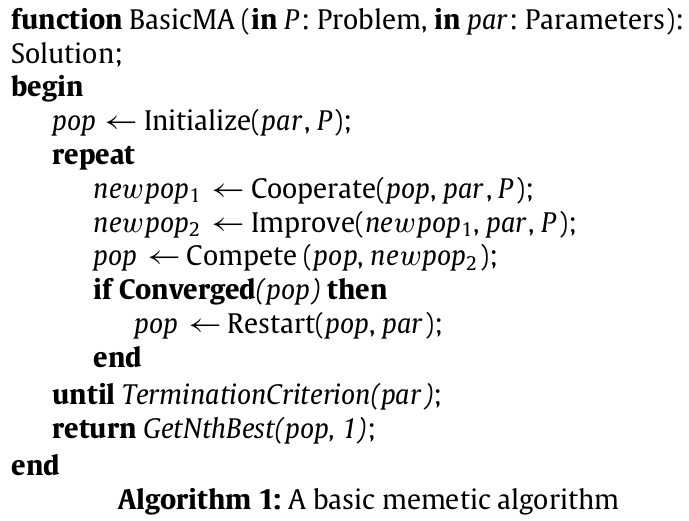
\includegraphics[width = 0.7\textwidth]{alg1.png}
    \caption{}
  	\end{figure}
 	
 } 
  \only<2>
 {
 The Initialize procedure
is responsible for producing the initial set of $|pop|$ solutions.
This could be done at random, but it is typical
for MAs to attempt to use high-quality solutions as starting point, either using some constructive heuristic, or by using a local-search procedure to
improve random solutions:\\
    \begin{figure}
    \centering
    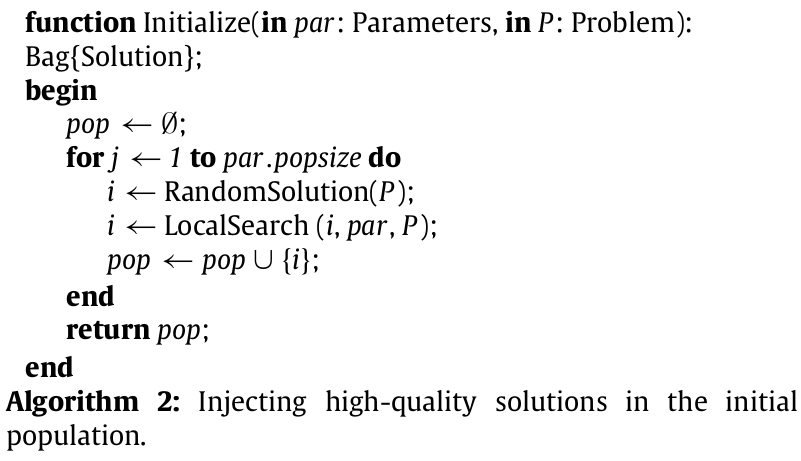
\includegraphics[width = 0.7\textwidth]{alg2.png}
    \caption{}
  	\end{figure}
 	
 } 
 \only<3>
 {
The procedures \emph{Cooperate} and \emph{Improve} constitute the core of
the MA. \emph{Cooperate} arises from the use of two operators for selecting solutions from the
population and recombining them, it can
be easily extended to use a larger collection of variation operators.\\
\vspace{0.15cm}
    \begin{figure}
    \centering
    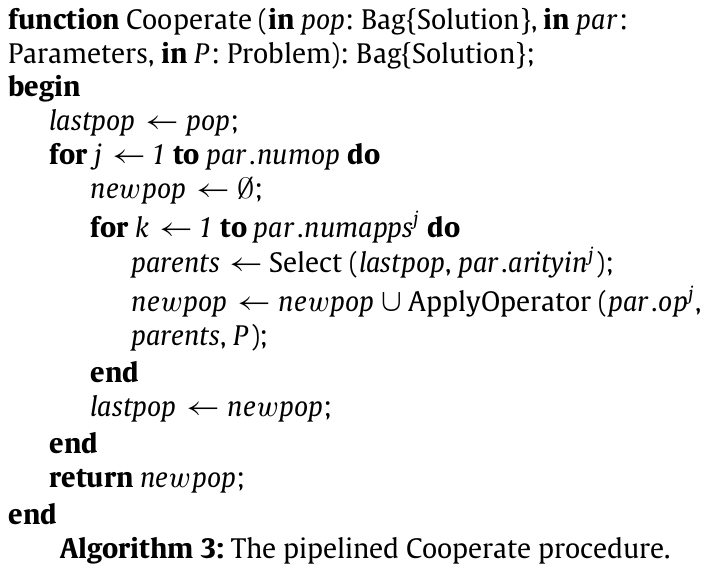
\includegraphics[width = 0.6\textwidth]{alg3.png}
    \caption{}
  	\end{figure}

 }
 
 \only<4>
 {
 \emph{Improve} embodies the application of
a local search procedure to solutions in the population, considering that for continuous optimization, the neighborhood $N(s)$ of a solution $s$ is an hypersphere with center $s$ ans radius equal to $\epsilon$ with $\epsilon>0$.\\
\vspace{0.15cm}
Hence, one have $N(s)=\{s' \in \Re^n : \parallel s'-s\parallel <\epsilon\}$ where $\parallel s'-s\parallel$ is the Euclidiean norm.\\
  
    \begin{figure}
    \centering
    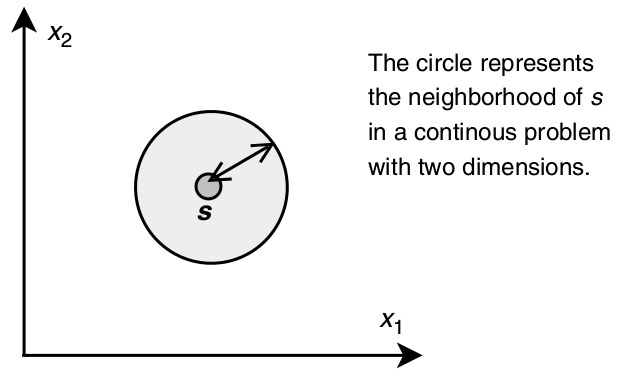
\includegraphics[width = 0.6\textwidth]{ls.png}
    \caption{}
  	\end{figure}

 }
 
 \only<5>
 {
The \emph{Compete} procedure is used to reconstruct the current
population using the old population $pop$ and the population of
offspring $newpop2$. There exist two main
possibilities for this purpose: the \textit{plus strategy} and the \textit{comma
strategy}:
	\vspace{0.5cm}
	\begin{enumerate}
	\item Plus Strategy: The current population is constructed taken the best popsize configurations from $pop \cup newpop$.\\
		\vspace{0.5cm}
	\item Comma Strategy: The best popsize configurations are taken just from newpop. In this case, it is required to have $|newpop| >popsize$, so as to put some selective pressure on the process.\\
	\end{enumerate}
 }
 \only<6>
 {
I order to apply a restart procedure, it must be decided whether the population has
degraded or has not, using some measure of information diversity
in the population. A very typical strategy is to
keep a fraction of the current population, and generate new (random
or heuristic) solutions to complete the rest.\\

    \begin{figure}
    \centering
    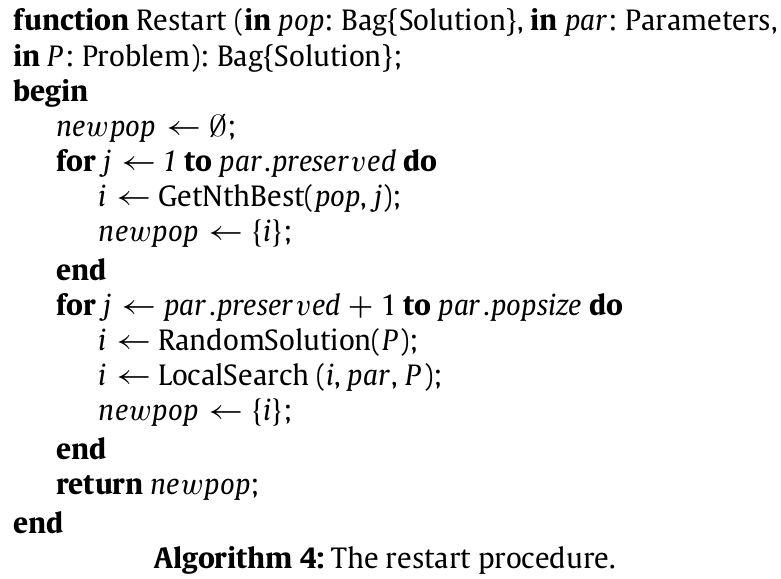
\includegraphics[width = 0.6\textwidth]{alg4.png}
    \caption{}
  	\end{figure}
  	
 }
 \only<7>
 {
  As for the \textit{TerminationCriterion} function, one of the following criteria could be used:\\
  \vspace{0.5cm}
   \begin{enumerate}
   \item Checking a limit on the total number of iterations.
   \item Reaching a maximum number of iterations without improvement.
   \item Having performed a certain number of population restarts.
   \item Reaching a certain target fitness.
   \end{enumerate}
 }
}

\section{Problem Description}

\frame {
  \frametitle{Problem Description}
  
 \only<1>
 {
 $\textbf{Four-bar Mechanism}$\\
\vspace{0.5cm}

\begin{columns}[T]
    \begin{column}{.5\textwidth}
    The objective is that the terminal $C$ reches as much as possible a set of target points $\{C_d^i\}$.\\
    \vspace{0.5cm}
     The engine torque is in $\theta_2$, while $r_1,r_2,r_3,r_4,r_{cx},r_{cy},x_0,y_0$ and $\theta_0$ are design parameters to be optimized.\\
	\vspace{0.5cm}
	Given all these parameters, it is possible to calculate the coordinates of the terminal $C$.\\
    \end{column}
    
    \begin{column}{.5\textwidth}
    
   \begin{figure}
    \centering
    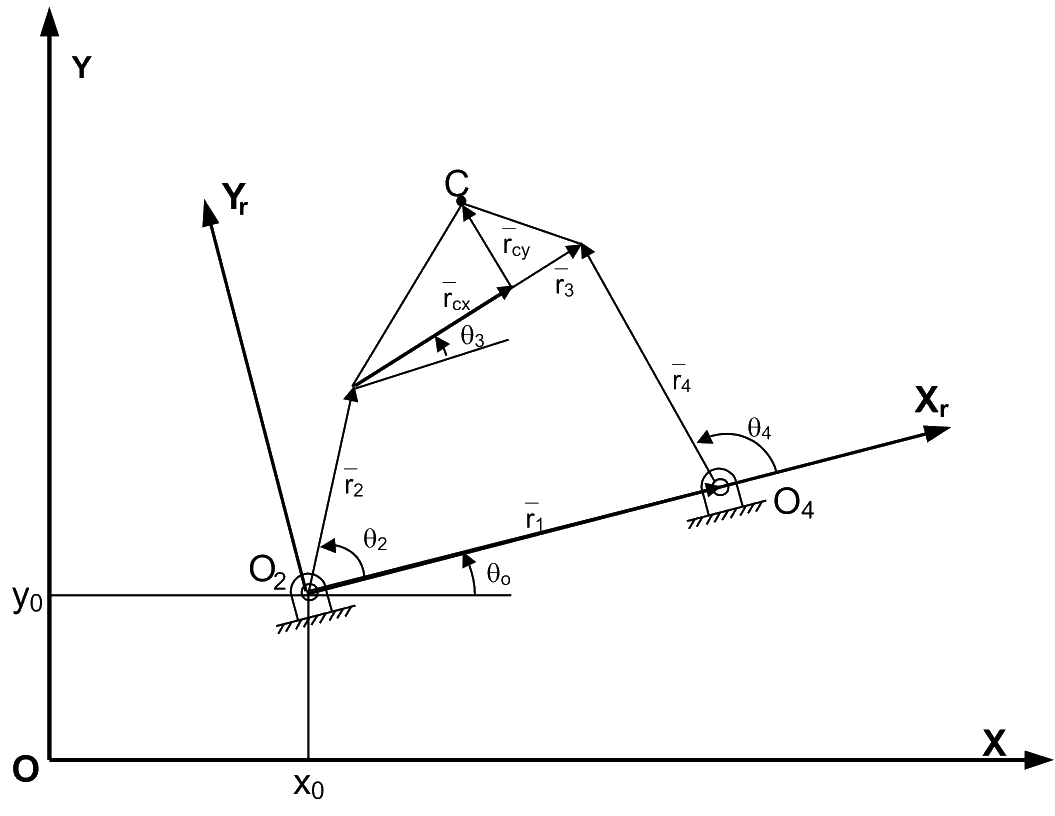
\includegraphics[width = 1.0\textwidth]{mecha.png}
    \caption{}
  \end{figure}
  
    \end{column}
  \end{columns}
 }
 \only<2>
 {
 $\textbf{Four-bar Mechanism}$\\
\vspace{0.5cm}

\begin{columns}[T]
    \begin{column}{.5\textwidth}
    With respect to the coordinate system in $x_0$, $y_0$ and $\theta_0$:\\
    \vspace{0.5cm}
    $\widehat{C}_r=\widehat{r}_2+\widehat{r}_{cx}+\widehat{r}_{cy}$
    $C_{xr}=r_2 \cos \theta_2 + r_{cx} \cos \theta_3 - r_{cy} \sin \theta_3$
    $C_{yr}=r_2 \sin \theta_2 + r_{cx} \sin \theta_3 + r_{cy} \cos \theta_3$\\
    \vspace{0.5cm}
    Transforming to the coordinate system \textbf{O}xy:\\
	\vspace{0.5cm}
	
	\begin{small}
 	$\begin{bmatrix}
 	C_x \\
 	C_y 
 	\end{bmatrix}=
 	\begin{bmatrix}
 	\cos \theta_0 & - \sin \theta_0 \\
 	\sin \theta_0 & \cos \theta_0
 	\end{bmatrix}
 	\begin{bmatrix}
 	C_{xr} \\
 	C_{yr} 
 	\end{bmatrix}+
 	\begin{bmatrix}
 	x_0 \\
 	y_0 
 	\end{bmatrix}$   
    \end{small}
    
    \end{column}
    
    \begin{column}{.5\textwidth}
    
   \begin{figure}
    \centering
    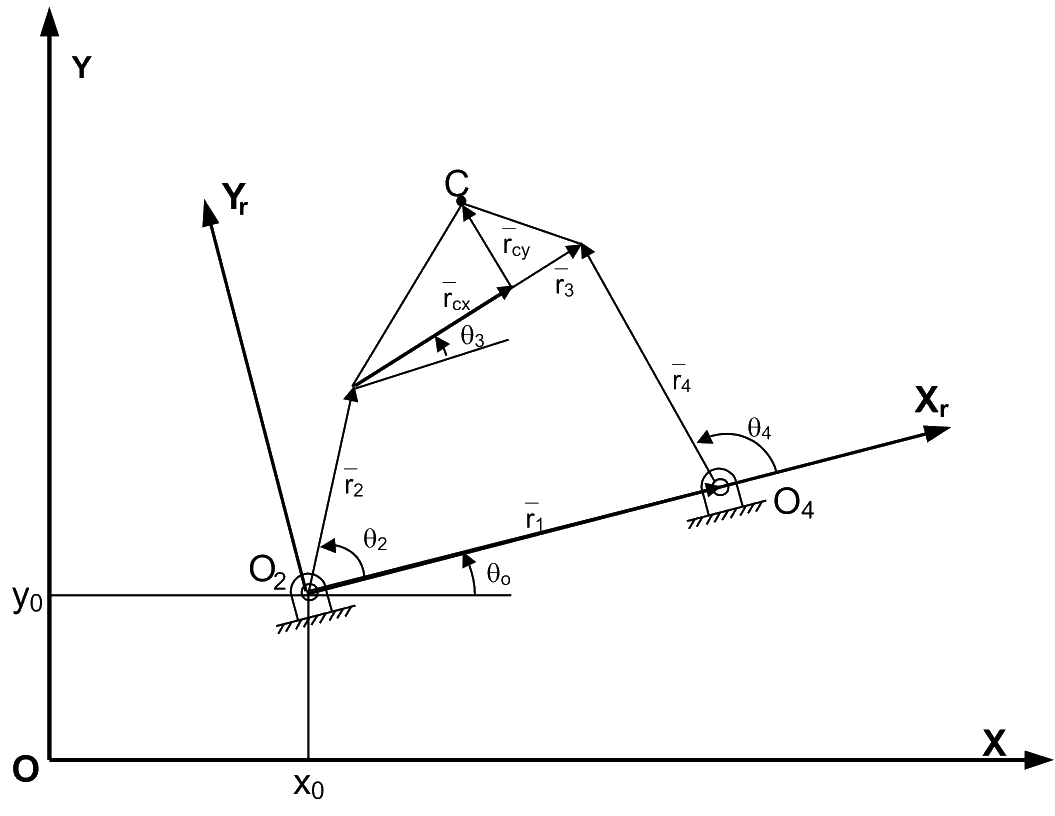
\includegraphics[width = 1.0\textwidth]{mecha.png}
    \caption{}
  \end{figure}
  
    \end{column}
  \end{columns}
 }
 \only<3>
 {
 $\textbf{Four-bar Mechanism}$\\
\vspace{0.5cm}

\begin{columns}[T]
    \begin{column}{.5\textwidth}
	Close loop Equations for the Mechanism:\\
	\vspace{0.5cm}
	
	$\widehat{r}_1+\widehat{r}_4=\widehat{r}_2+\widehat{r}_3$	
	$r_2 \cos \theta_2 +r_3 \cos \theta_3=r_1 +r_4 \cos \theta_4$
	$r_2 \sin \theta_2 +r_3 \sin \theta_3=r_4 \sin \theta_4$
	
	\vspace{0.5cm}
	squaring both equations:\\
	\vspace{0.5cm}
	
	$r_4^2 \cos^2 \theta_4=(r_2 \cos \theta_2 +r_3 \cos \theta_3-r_1)^2$
	$r_4^2 \sin^2 \theta_4=(r_2 \sin \theta_2 +r_3 \sin \theta_3)^2$\\
	
    \end{column}
    
    \begin{column}{.5\textwidth}
    
   \begin{figure}
    \centering
    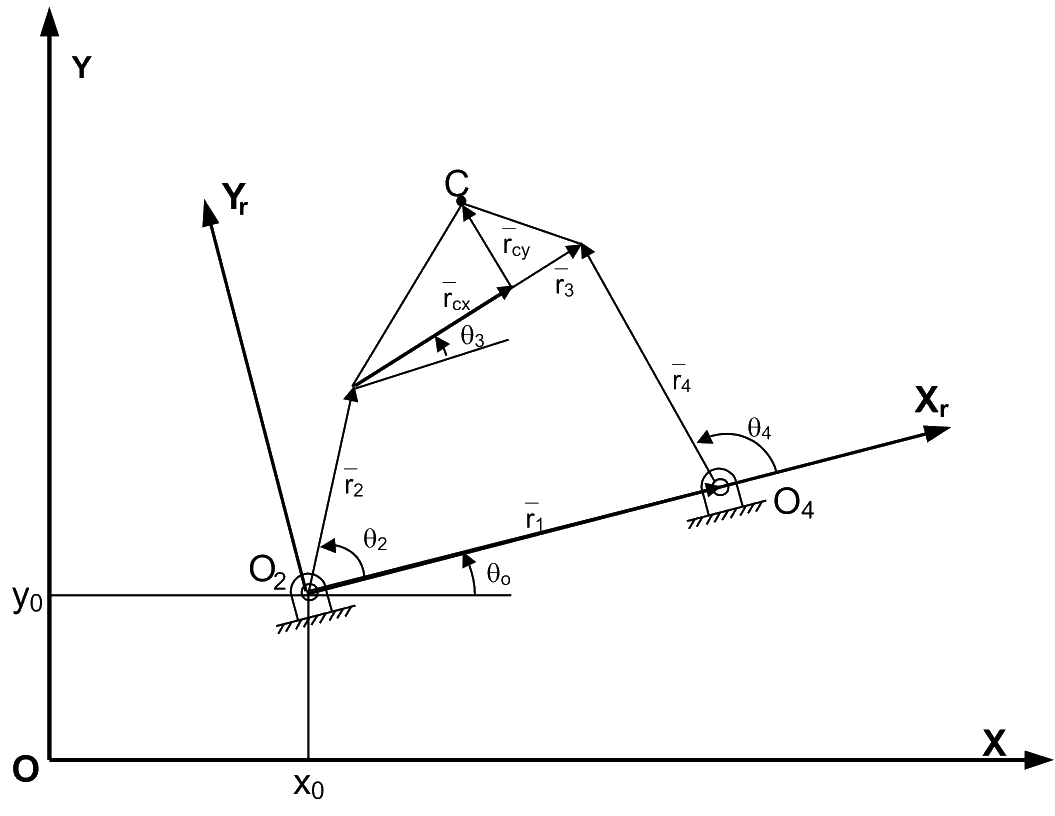
\includegraphics[width = 1.0\textwidth]{mecha.png}
    \caption{}
  \end{figure}
  
    \end{column}
  \end{columns}
 }
 \only<4>
 {
 	By summing the equations and applying trigonometric identities we obtain:\\
 	\vspace{0.5cm}
 	$r_4^2 = r_1^2 + r_2^2 + r_3^2 + 2r_2 r_3 \cos(\theta_2-\theta_3)- 2 r_1 r_3 \cos \theta_3 -2r_1 r_2 \cos \theta_2$\\
 	\vspace{0.5cm}
 	By rearranging and redefining terms we formulate the expresion called \emph{Freudenstein's Equation}:

	$$k_1 \cos \theta_3 + k_2 \theta_2 + k_3 = \cos (\theta_2 - \theta_3)$$
	Where:
	$$k_1=\frac{r_1}{r_2};~~ k_2=\frac{r_1}{r_3};~~ k_3=\frac{r_4^2-r_1^2 - r_2^2 - r_3^2}{2r_2 r_3}$$
 	
 }
 \only<5>
 {
 Let be $\varphi=tan (\frac{\theta_3}{2})$, then
 
 $$\sin \theta_3 = \frac{2 \varphi}{1+\varphi^2};~~~ \cos \theta_3= \frac{1-\varphi^2}{1+\varphi^2}$$\\
 
 \vspace{0.5cm}
 Substituing in the Freudenstein Equation and rearranging terms:\\
 
 $$k_1(\frac{1-\varphi^2}{1+\varphi^2})+ k_2 \cos \theta_2 + k_3 = (\frac{1-\varphi^2}{1+\varphi^2}) \cos \theta_2 + \frac{2 \varphi}{1+\varphi^2} \sin \theta_2$$
 $$\varphi^2[k_3+(k_2+1)\cos \theta_2 -k_1]+ \varphi(-2\cos \theta_2) + [k_1+(k_2-1)\cos \theta_2 + k_3]=0$$ 
 
 $$\Rightarrow \varphi=\frac{-b\pm \sqrt{b^2-4ac}}{2a}$$
 }
 \only<6>
 {
 Where:\\
 \vspace{0.5cm}
 $~~~~a=k_3+(k_2+1)\cos \theta_2 -k_1$\\
 $~~~~b=-2\cos \theta_2$\\
 $~~~~c=k_1+(k_2-1)\cos \theta_2 + k_3$\\
 \vspace{0.5cm}
 Then, $\theta_3$ can be computed as $\theta_3=2tan^{-1} \varphi$\\
 \vspace{0.5cm}
 If $\varphi \not\in \Re$, the mechanism cannot be constructed with the given configurations.\\
 
 }
 }

\section{Implementation}

\frame {
  \frametitle{Implementation}
 \only<1>
 {
 $\textbf{Mechanism Restrictions.}$\\
 \vspace{0.5cm}
 \begin{enumerate}
   \item Input angles $\theta_2^i$ should be arranged such that they are consecutive in a $2\pi$ radians circunference.
 \item All link magnitudes shall be positive: $r_1,r_2,r_3,r_4,r_{cx},r_{cy}>0$.
 \item Grashof Condition imposed to form a \emph{Crank-Rocker} configuration, that is $r_1+r_2<r_3+r_4$, with $r_2<r_3,r_4<r_1$, and the shortest link is connected to the base.
   \begin{figure}[H]
    \centering
    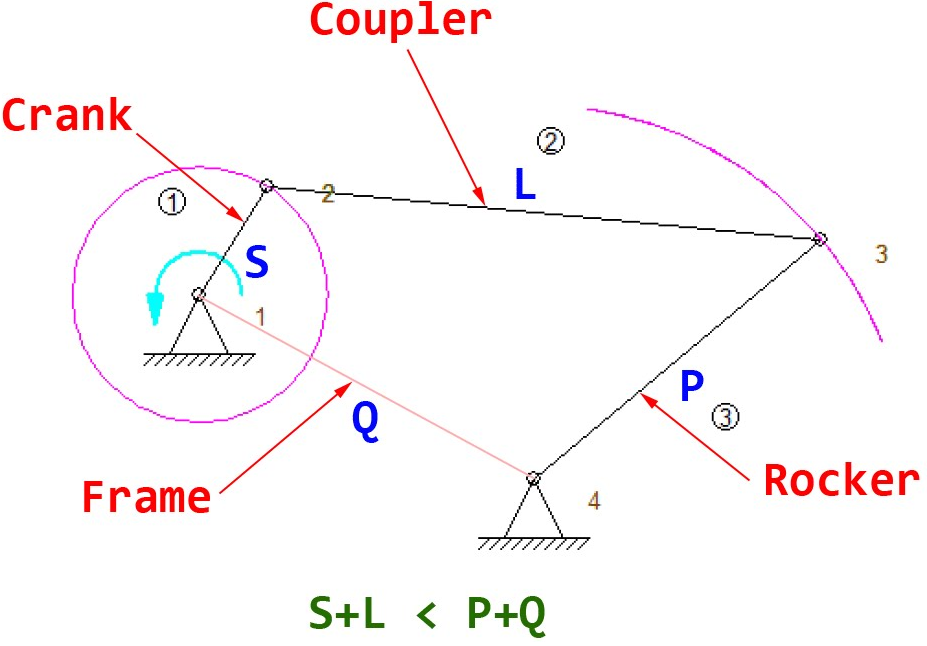
\includegraphics[width = 0.4\textwidth]{grashof.png}
    \caption{}
  \end{figure}

 \end{enumerate}
 }
 \only<2>
 {
In order to use this definition of the problem when the optimization algorithm is implemented, the constraints 1,2 \& 3 are retained when values are assigned to design variables, and also they are inserted into the goal function as penalty functions as follows:
$$min\{[(C_{xd}^i(X)-C_{x}^i(X))^2+(C_{yd}^i(X)-C_{y}^i(X))^2]+M_1 h_1 (X) + M_2 h_2 (X)\}$$
where:\\
$X=[r_1,r_2,r_3,r_4,r_{cx},r_{cy},\theta_0,\theta_2^1,\theta_2^2,...,\theta_2^N]$\\
 \vspace{0.5cm}
$h_1(X) \in \{0,1\} \rightarrow$ Grashof Condition true/false.\\
$h_2(X) \in \{0,1\} \rightarrow$ Sequence Condition for $\theta_2$ true/false.\\
 \vspace{0.5cm}
and $M_1$ and $M_2$ are constants of a very high value that penalize the goal function when the associated constraint fails.
 }
 
 \only<3>
 {
 	Implemented Operators:\\
 \vspace{0.5cm}

\textbf{Recombination.} It can be defined as a process in which a set $S_{par}$ of $n$ configurations (parents) is manipulated to create a set $S_{desc} \subseteq sol_P (x)$ of $m$ new configurations (descendants). \\
 \vspace{0.5cm}
The creation of these descendants involves the identification and combination of features extracted from the
parents. In this implementation we use the \emph{Dynastically Optimal Recombination} scheme, in which every recombination is explored in order to find the best configuration, the result will be at least equal to the best parent. \\
 \vspace{0.5cm}
We are also considering a partial recombination, that is, we are only considering blocks of information when recombining individuals, namely, the sets $\{r_1,r_2,r_3,r_4\}$, $\{r_{cx},r_{cy}\}$, $\{x_0,y_0,\theta_0\}$ and $\{\theta_2^1,\theta_2^2,...,\theta_2^N\}$\\
 }  
 \only<4>
 {
 \textbf{Mutation.} It creates a single offspring $x'_i$ from each parent $x_i$, $\forall i \in \{1,2,...,popsize\}$ by
 $$x'_i(j)=x_i(j)+\epsilon N_j(0,1)$$
 where $j$ is a random integer $\in \{1,2,...,popsize\}$, and $N_j(0,1)$ is a random value generated from a standard normal distribution.
  
 }  

}

\section{Results}

\frame {
  \frametitle{Results}
 \only<1>
 {
 The following table shows the best results obtained from 100 executions of the algorithm.\\
  \vspace{0.5cm}
 Target points: $C_d^i=\{(20,20),(20,25),(20,30),(20,35),(20,40),(20,45)\}$\\
 Limits: $r_1,r_2,r_3,r_4,r_{cx},r_{cy},x_0,y_0 \in [0,60]$; $\theta_0,\theta_2^1,\theta_2^2,\theta_2^3,\theta_2^4,\theta_2^5,\theta_2^6 \in [0,2\pi]$\\
 Parameters: $popsize=100$, $MaxIte=1000$, $\epsilon_r=10$, $\epsilon_{\theta}=0.1$\\
   \begin{figure}[H]
    \centering
    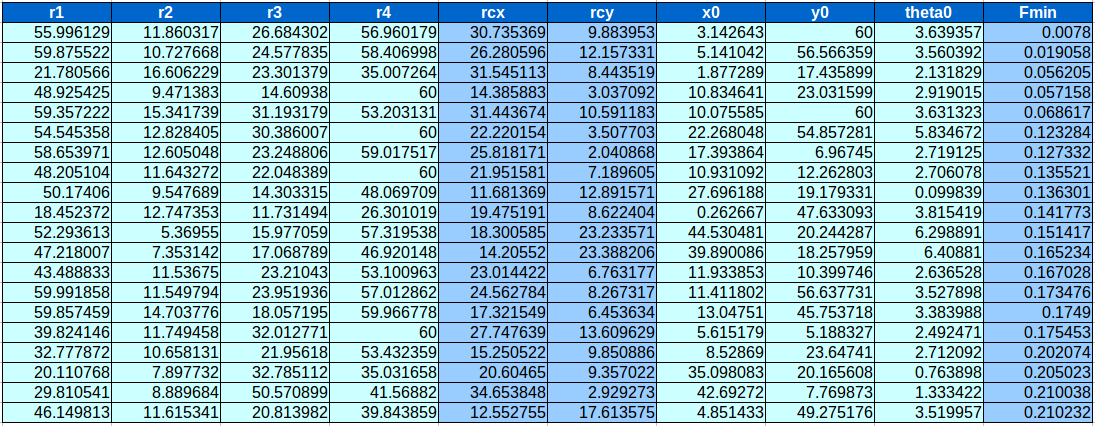
\includegraphics[width = 1.0\textwidth]{tabla.png}
    \caption{}
  \end{figure}
	
 }
}


  
\section{Bibliography}

\begin{frame}{Bibliography}
\bibliographystyle{plainnat}
\bibliography{BIB}
\frametitle{References}
\begin{itemize}

\begin{small}

\item[1]
{\it J.A. Cabrera \& A. Simon, M. Prado} (2002).
{\bf Optimal synthesis of mechanisms with genetic algorithms.} Journal of Mechanism and Machine Theory 37 (2002) 1165-1177.

\vspace{0.2cm}

\item[2]
{\it El-Ghazali Talbi} (2009).
{\bf Metaheuristics: form Design to Implementation.} John Wiley \& Sons, Inc.

\vspace{0.2cm}

\item[3]
{\it Pablo Moscato \& Carlos Cotta} (2003).
{\bf A Gentle Introduction to Memetic Algorithms.} Handbook of Metaheuristics, Kluwer
Academic Publishers, pp. 105-144

\vspace{0.2cm}

\item[4]
{\it Kumar Chellapilla} (1998).
{\bf Combining Mutation Operators in Evolutionary Programming.} IEEE Transactions on Evolutionary Computation, Vol. 2, No. 3.

\vspace{0.2cm}

\item[5]
{\it Ferrante Neri \& Carlos Cotta} (2012).
{\bf Memetic algorithms and memetic computing optimization: A literature review.} Swarm and Evolutionary Computation 2, 1–14.

\end{small}
\end{itemize}
\end{frame}

\end{document}